YOLO26n-MHSA được dẫn xuất từ YOLO26n bằng một thay đổi cục bộ trong đường tổng hợp đặc trưng, thay vì thiết kế lại toàn bộ detector. Kiến trúc YOLO26n gốc chủ yếu dựa trên các khối tích chập để trích xuất mẫu thị giác cục bộ và hợp nhất đặc trưng đa tỉ lệ trước lớp \textit{Detect}. Thiết kế này hiệu quả về tính toán, nhưng hành vi trong lớp học thường phụ thuộc vào quan hệ không gian xa, ví dụ tương quan giữa tư thế đầu, vị trí tay, vùng bàn học và vật thể nhỏ như điện thoại hoặc vở.

\begin{figure}[htbp]
  \centering
  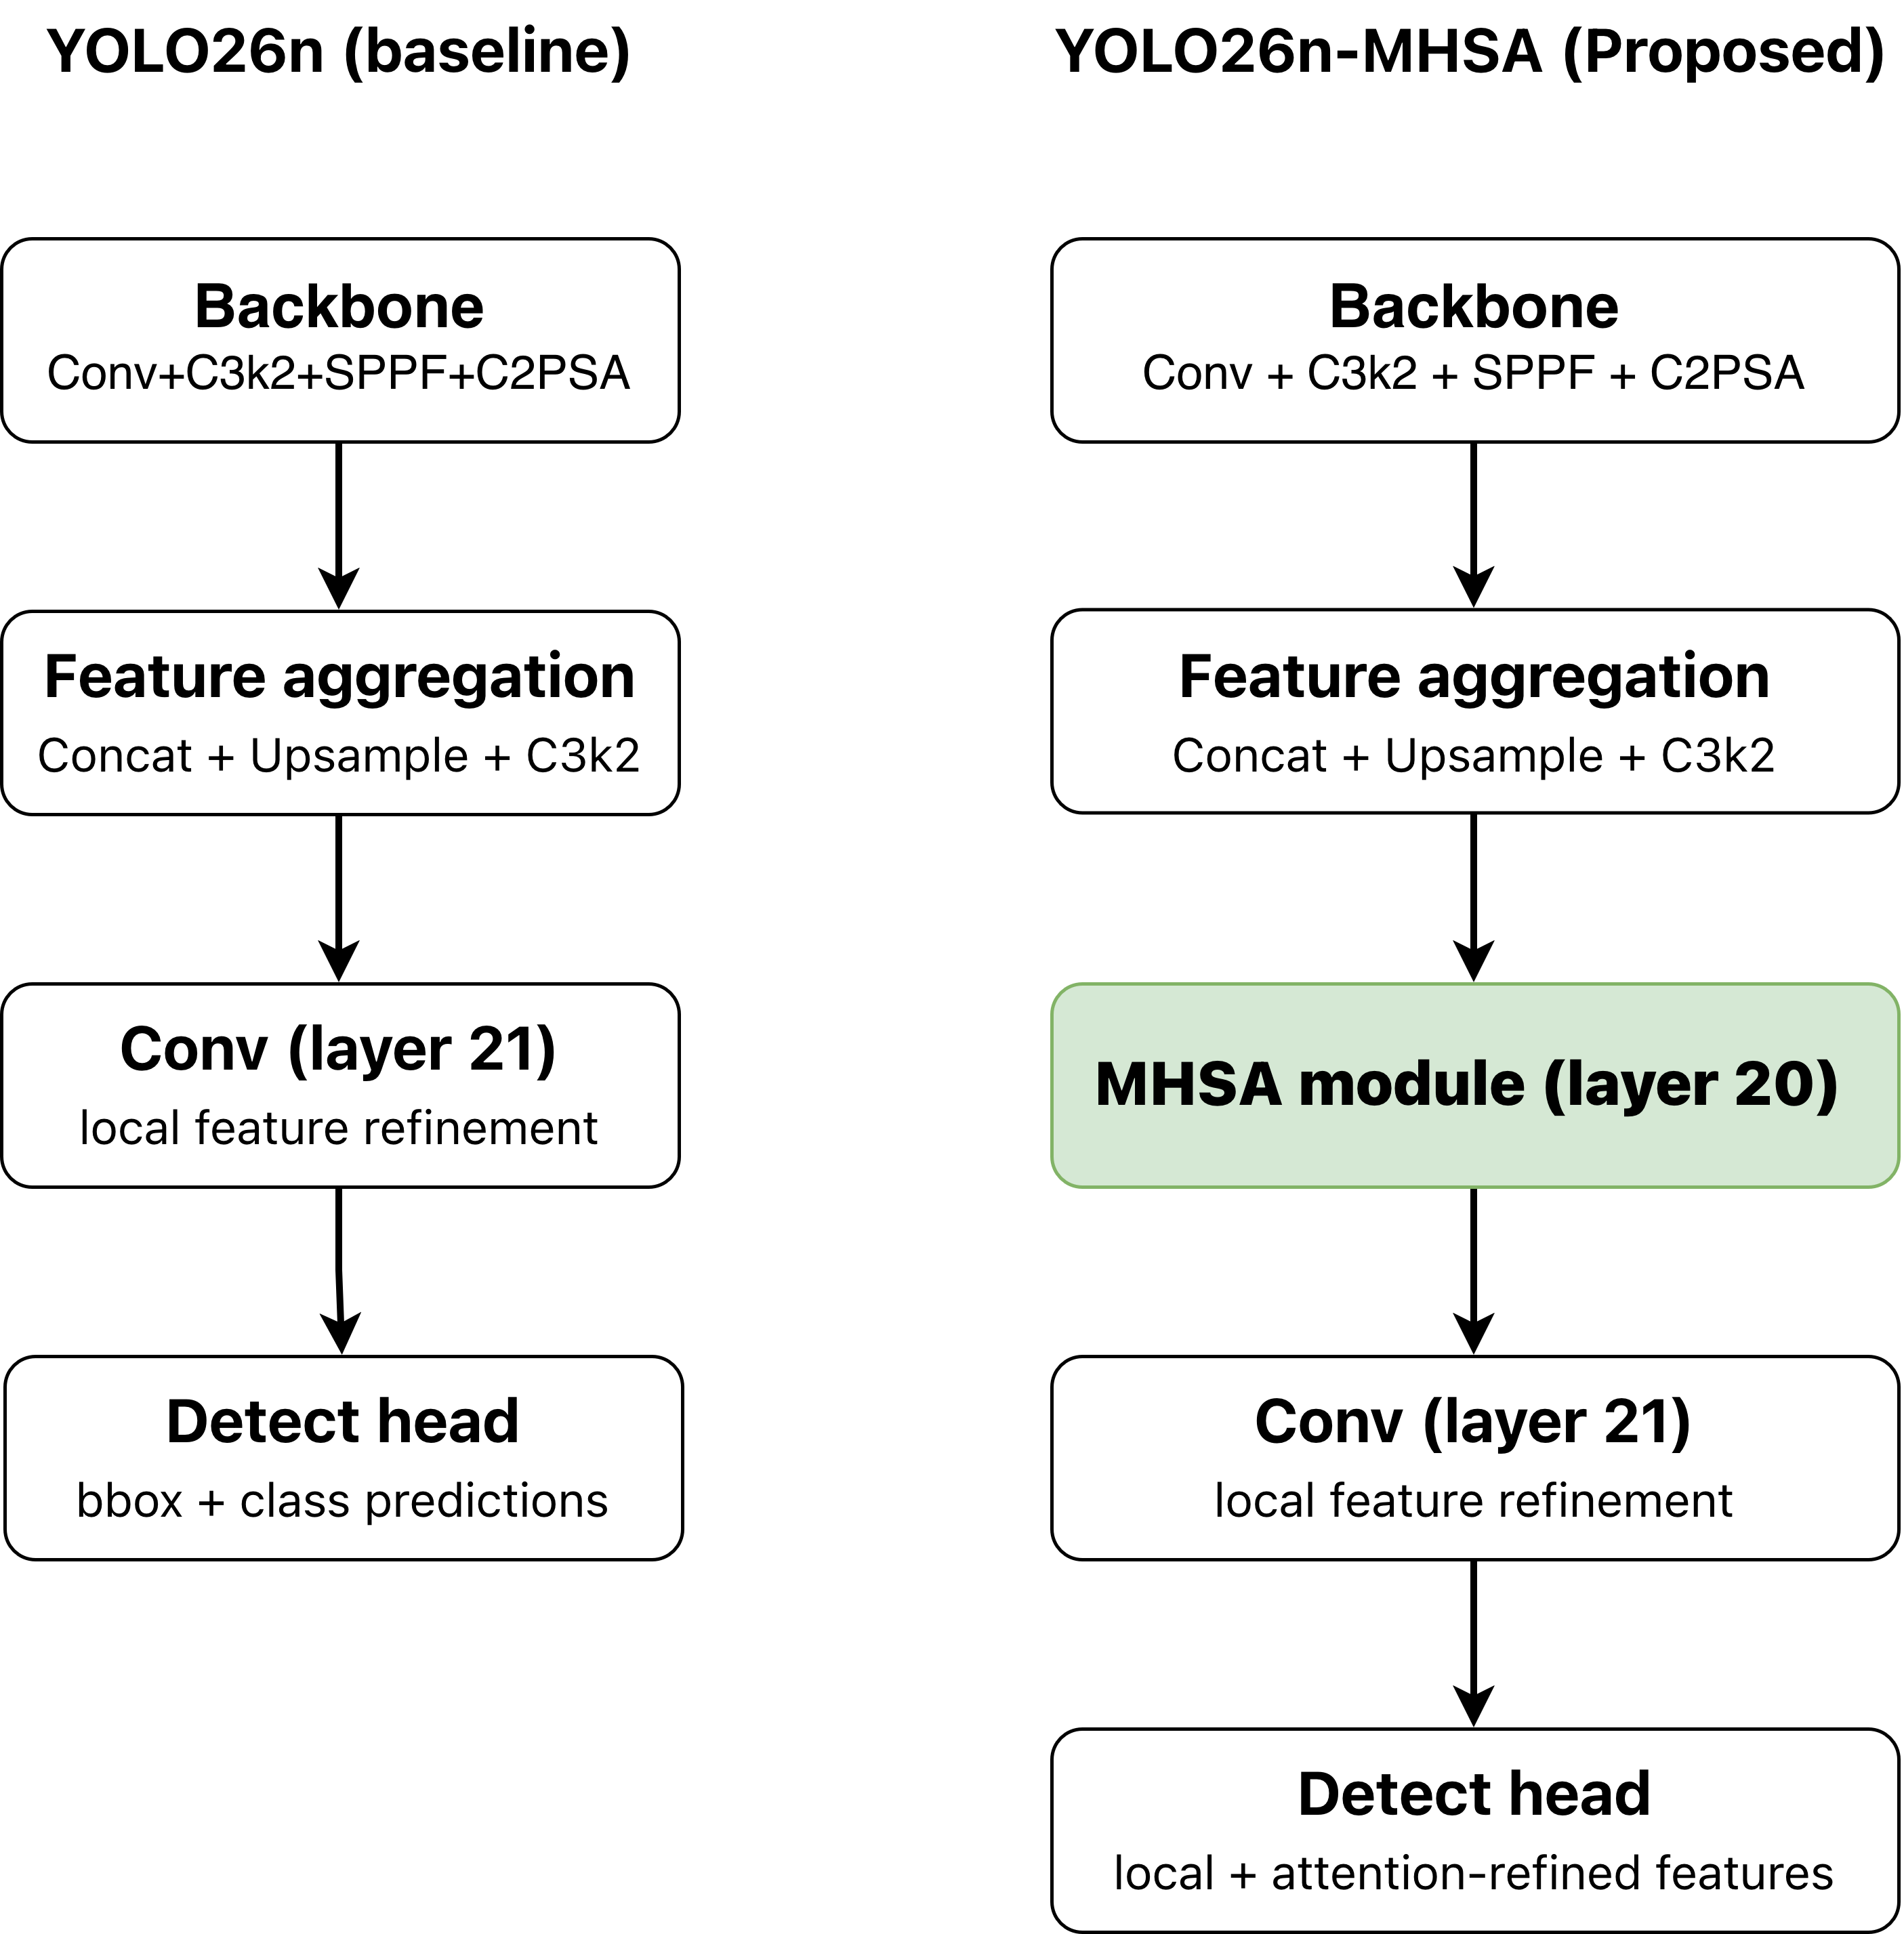
\includegraphics[width=0.9\textwidth]{figures/yolo.png}
  \caption{So sánh cấu trúc giữa detector YOLO26n gốc và biến thể YOLO26n-MHSA. Biến thể đề xuất chèn một khối MHSA vào head phát hiện để bổ sung ngữ cảnh không cục bộ trước lớp phát hiện cuối.}
  \label{fig:yolo-mhsa}
\end{figure}

Hình~\ref{fig:yolo-mhsa} trình bày khác biệt cấu trúc trước và sau khi thêm Multi-Head Self-Attention. Trong YOLO26n-MHSA, backbone và hầu hết kết nối trong head phát hiện được giữ nguyên. Thay đổi chính là chèn một khối MHSA sau khối C3k2 tại layer 19 và trước lớp tích chập tiếp theo tại layer 21. Nhánh đặc trưng đã tăng cường attention sau đó tiếp tục được đưa tới lớp \textit{Detect} cùng các đặc trưng ở tỉ lệ khác. Cách đặt này cho phép detector tinh chỉnh một nhánh đặc trưng trung gian bằng ngữ cảnh toàn cục nhưng vẫn giữ luồng đặc trưng YOLO đa tỉ lệ và backbone nhẹ. Cấu hình YAML đầy đủ của biến thể này được trình bày trong Phụ lục~\ref{appendix:yolo26n-mhsa-yaml}.

Lý do chọn thay đổi cục bộ là để giữ thí nghiệm so sánh có kiểm soát. Nếu thay đổi đồng thời backbone, neck, head và chiến lược huấn luyện, rất khó xác định phần cải thiện đến từ đâu. Trong thiết kế này, phần lớn kiến trúc YOLO26n được giữ nguyên; do đó khác biệt hiệu năng giữa YOLO26n và YOLO26n-MHSA có thể quy chủ yếu cho mô-đun MHSA được thêm vào. Điều này phù hợp với mục tiêu của đồ án: khảo sát vai trò của attention đối với nhận diện hành vi lớp học trong bối cảnh nhiều đối tượng và nhiều che khuất.

Gọi \(F\in\mathbb{R}^{H\times W\times C}\) là bản đồ đặc trưng đi vào mô-đun MHSA, trong đó \(H\), \(W\) và \(C\) lần lượt là chiều cao, chiều rộng và số kênh. Bản đồ đặc trưng được làm phẳng thành chuỗi token
\begin{equation}
\label{eq:mhsa-flattened-features}
    Z\in\mathbb{R}^{N\times C}, \qquad N=H\times W.
\end{equation}
Từ \(Z\), mô-đun tính các ma trận query, key và value:
\begin{equation}
\label{eq:mhsa-projections}
    Q=ZW_Q, \qquad K=ZW_K, \qquad V=ZW_V.
\end{equation}
Với một attention head, scaled dot-product attention được tính bởi
\begin{equation}
\label{eq:scaled-dot-product-attention}
    \operatorname{Attention}(Q,K,V)=\operatorname{softmax}\left(\frac{QK^\top}{\sqrt{d}}\right)V,
\end{equation}
trong đó \(d\) là chiều của vector query và key. Với \(h\) head song song, đầu ra của các head được ghép và chiếu tuyến tính:
\begin{equation}
\label{eq:mhsa-output}
    \operatorname{MHSA}(Z)=\operatorname{Concat}(head_1,head_2,\ldots,head_h)W_O.
\end{equation}
Một kết nối tắt được dùng để bảo toàn biểu diễn ban đầu:
\begin{equation}
\label{eq:mhsa-residual}
    Z' = Z + \operatorname{MHSA}(Z).
\end{equation}
Sau đó \(Z'\) được reshape lại thành bản đồ đặc trưng không gian và truyền tới các lớp còn lại của head.

Về mặt trực giác, MHSA cho phép một vị trí đặc trưng ở vùng đầu, tay hoặc bàn học trao đổi thông tin với các vùng xa hơn trước khi detector dự đoán hộp và nhãn. Điều này đặc biệt hữu ích với các hành vi có tín hiệu phân tán, chẳng hạn viết bài phụ thuộc vào cả tư thế tay và vùng vở, hoặc sử dụng điện thoại phụ thuộc vào vật thể nhỏ trong tay và tư thế nhìn xuống. Tuy nhiên, vì chỉ thêm một nhánh attention, mô hình vẫn giữ được tính nhẹ của YOLO26n và phù hợp với pipeline video.

Đầu ra của YOLO26n-MHSA ở mỗi khung hình là tập hộp phát hiện kèm nhãn hành vi và điểm tin cậy. Các nhãn này được giữ thống nhất trong toàn pipeline; việc ánh xạ nhãn giữa bộ dữ liệu Local và SCB chỉ được thực hiện trong thiết lập thực nghiệm. Phần method vì vậy xem detector như nguồn tạo bằng chứng quan sát, còn mọi diễn giải phía sau phải tính đến khả năng detector bỏ sót hoặc nhận nhầm hành vi.